\subsection{Matched Strong Controls and Versioned Consumer Contracts}\label{app:completion_controls}

This retrospective completion uses all ten saved fresh-confirmation checkpoints
and a fixed plan published before the additional computations. It leaves the
original development choice, confirmation bank and verdicts unchanged.
From the earlier development grid, we choose the feature-map coefficient with
the lowest reconstruction ratio among candidates with mean primary difference
within $0.5$ points of detachment, mean reconstruction ratio at most $0.95$,
and disagreement at most $5\%$ on every development seed. This utility-aware
rule selects $\lambda=1$; the earlier compatibility-only rule selected
$0.01$ and failed its primary gate. Both decisions remain reported.
The new branch starts from each saved healthy model and Adam state and uses
the same $30$ epochs, reconstruction dose $100$ and future minibatches.
Both nonlinear encoder layers update. The full-feature map is folded into
the float32 legacy reader for serving.

We also fit the same standardized OLS reader on detached, joint, distilled and
feature-aligned endpoints. Every fit uses fitting-set features and healthy
teacher logits, without labels, test inputs or a coefficient search. The
previously saved OLS reader and its identical new fit are counted once in
comparisons: $100$ recorded endpoints contain $90$ distinct model/reader pairs.
Learned and OLS readers use their actual float32 serving weights; raw detached
and joint readers retain the original float64 diagnostic interface.

\begin{table}[H]
\centering
\caption{Matched HAR completion on the ten saved fresh-confirmation seeds. This retrospective comparison uses development-selected full-feature alignment and training-only OLS; no test fitting or coefficient search. Primary values are paired percentage-point differences to detachment. Each changed/certified cell reports mean disagreement and the number of new $1{,}024$-monitor bounds below $5\%$, with tail $0.05/1{,}000$. Selective consumers use fixed healthy-training confidence thresholds targeting $80\%$ or $50\%$ coverage. These new bounds do not replace the earlier confirmation.}
\label{tab:completion_controls}
\footnotesize
\setlength{\tabcolsep}{3pt}
\begin{tabular}{lrrrrr}
\toprule
Arm & primary & MSE / D & class & selective 80 & selective 50 \\
\midrule
Detach & $+0.00\ [+0.00,+0.00]$ & $1.000$ & $3.71\%$; $3/10$ & $9.64\%$; $0/10$ & $17.64\%$; $0/10$ \\
Detach + OLS & $+0.00\ [+0.00,+0.00]$ & $1.000$ & $0.93\%$; $10/10$ & $2.20\%$; $4/10$ & $2.67\%$; $3/10$ \\
Joint & $+0.02\ [-0.38,+0.43]$ & $0.767$ & $27.66\%$; $0/10$ & $52.71\%$; $0/10$ & $38.72\%$; $0/10$ \\
Joint + OLS & $+0.02\ [-0.38,+0.43]$ & $0.767$ & $3.22\%$; $0/10$ & $8.31\%$; $0/10$ & $9.85\%$; $0/10$ \\
Distilled head & $+0.30\ [-0.01,+0.61]$ & $0.780$ & $1.67\%$; $8/10$ & $4.71\%$; $0/10$ & $6.50\%$; $0/10$ \\
Distilled + OLS & $+0.30\ [-0.01,+0.61]$ & $0.780$ & $1.46\%$; $9/10$ & $3.52\%$; $0/10$ & $4.82\%$; $0/10$ \\
Feature align. ($\lambda=1$) & $+0.56\ [+0.24,+0.88]$ & $0.771$ & $1.92\%$; $8/10$ & $5.42\%$; $0/10$ & $7.23\%$; $0/10$ \\
Feature align. + OLS & $+0.56\ [+0.24,+0.88]$ & $0.771$ & $1.74\%$; $8/10$ & $4.15\%$; $0/10$ & $5.37\%$; $0/10$ \\
Logit map & $+0.42\ [+0.03,+0.80]$ & $0.777$ & $1.64\%$; $9/10$ & $4.59\%$; $0/10$ & $6.43\%$; $0/10$ \\
\bottomrule
\end{tabular}
\end{table}


The stronger feature-alignment baseline retains reconstruction progress
(MSE $\CompleteFeatureMse$ of detachment) with primary difference
$+\CompleteFeatureGain$ points $[\CompleteFeatureGainLow,\CompleteFeatureGainHigh]$.
Full-feature alignment is therefore competitive with the distilled head. Unconstrained joint training followed
by OLS reaches $\CompleteJointOlsChanged\%$ mean class disagreement, versus
$\FreshDirectChanged\%$ for joint distillation. These intervals describe a retrospective matched comparison on the saved benchmark.

Decision disagreement counts several kinds of change. With labels available,
we report negative flips (healthy-correct to updated-wrong), positive flips,
and changes between two wrong classes~\citep{yan2021positive}. Their rates sum
to total disagreement, while the change in legacy accuracy equals
positive minus negative flips. Joint training's $27.66\%$ class disagreement
contains $22.97\%$ negative flips; OLS lowers those to
$\CompleteJointOlsNfr\%$. Joint distillation has
$\CompleteDirectNfr\%$ negative flips and $0.91\%$ positive flips. Total
agreement is a conservative compatibility contract, rather than a measure of
harmful changes alone.

For a probability-dependent consumer, define $q_\tau(x)=\arg\max_j p_j(x)$
when $\max_jp_j(x)\ge\tau$, and $q_\tau(x)=-1$ otherwise. We freeze two
thresholds at the $20$th and $50$th percentiles of healthy fitting-set confidence.
They target $80\%$ and $50\%$ fitting coverage; healthy test coverage is
$71.32\%$ and $42.65\%$. The new audit uses a fresh uniform $1{,}024$-input
monitor and tail $0.05/1{,}000$, covering the declared new reader/contract bank.
Its classification counts, including distilled $8/10$ and distilled-plus-OLS
$9/10$, are separate from the earlier $10/10$ confirmation under its original
monitor and $160$-consumer allocation. Neither monitor is selected by outcome.

\begin{figure}[htbp]
\centering
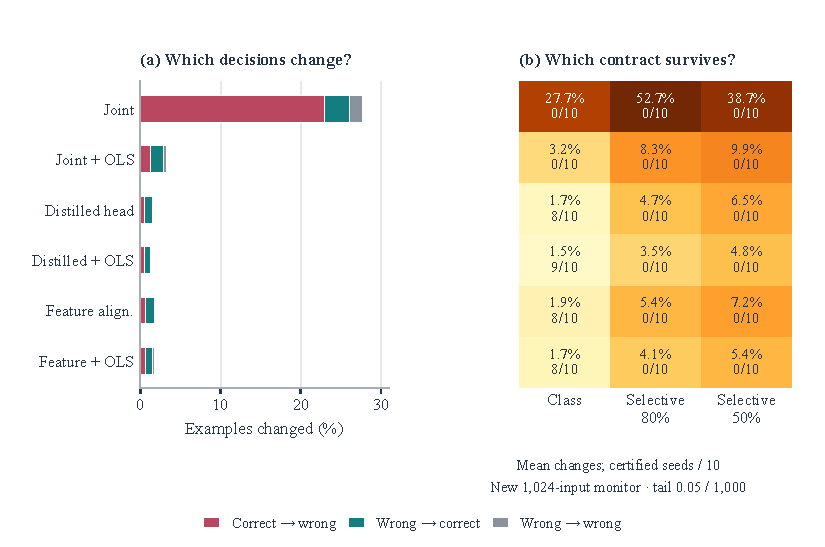
\includegraphics[width=\linewidth]{figures/fig_consumer_contracts.pdf}
\caption{Consumer-specific retention on the ten saved HAR seeds. Left: the
three disjoint contributions to class disagreement. Right: mean disagreement
and certified seed counts for the class decision and two fixed selective
consumers. Coverage labels name healthy-training targets, not test guarantees.
The new monitor and family allocation leave earlier confirmation counts intact.}
\label{fig:consumer_contracts}
\end{figure}

No tested reader certifies either selective consumer on all seeds. Among the
auxiliary-learning readers, every selective count is $0/10$; detached-plus-OLS
certifies $4/10$ and $3/10$, with no reconstruction gain. The distilled head's selective disagreement
is $4.71\%$ and $6.51\%$, versus $1.67\%$ for classification; OLS reduces
these to $3.51\%$ and $4.82\%$, without certifying the threshold contracts.
Distilled-head coverage is $69.14\%$ and $39.86\%$, and OLS coverage is
$70.61\%$ and $41.64\%$. Per-seed coverage, accepted-set accuracy, NLL, ECE,
flows and bounds are retained in the numerical records. Class agreement alone
does not retain probability-dependent decisions. Independent saved-state
replay checks predictions, flow decomposition, thresholded decisions and bounds.
An isolated native float32 audit returns both outputs in one encoder call.
At batch $1{,}024$, joint-plus-OLS, feature alignment and feature-plus-OLS cost
$1.064\times$, $1.057\times$ and $1.060\times$ current-only inference;
at batch one their ratios are $1.109\times$, $1.102\times$ and $1.110\times$.
The folded feature-map reader has the same $390$ serving parameters as the
direct distilled head; its $4{,}096$ map weights are needed only during training.
